\chapter{カレントミラーを組み合わせた折り返し型アナログ乗算回路}

    \section{回路構成}
        序論で述べたS/N比向上のための方針として、折り返しカスコードの構成をとることが考えられる。図\ref{fig:3_folded_gilbert}に折り返しカスコード型の乗算回路を示す。
        \begin{figure}[!b]
            \begin{center}
                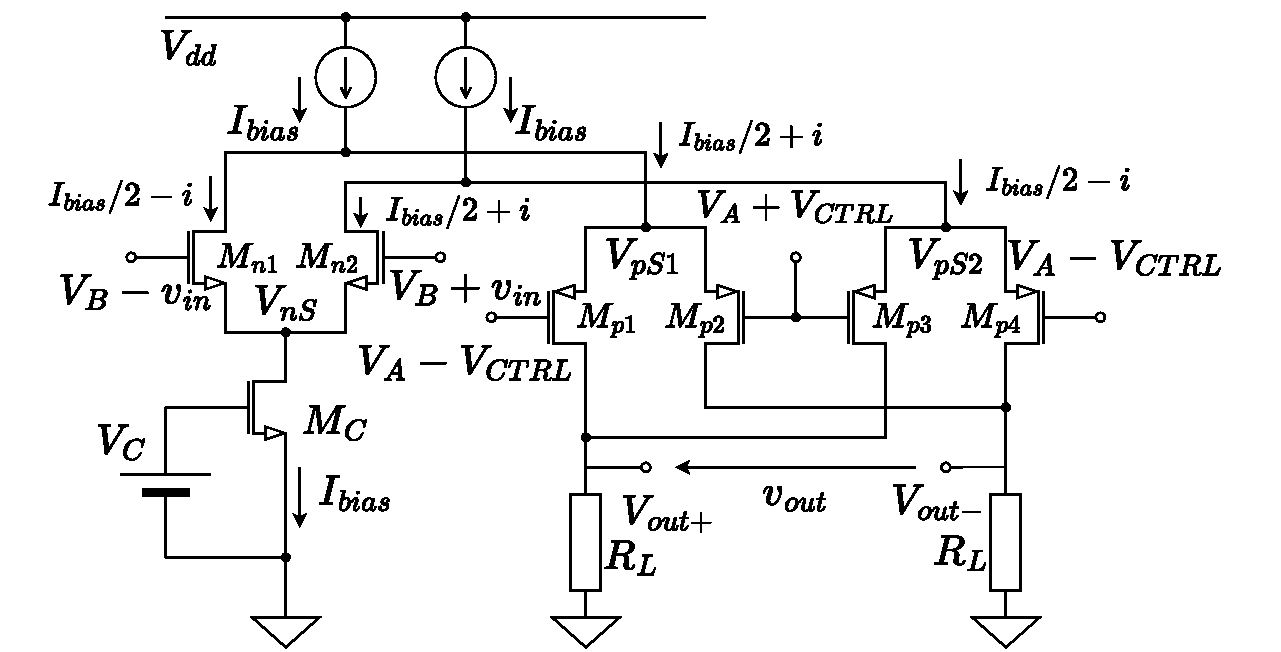
\includegraphics[width=0.99\linewidth]{figures/chapter3/folded_gilbert.pdf}
                \caption{折り返しカスコード型乗算回路}
                \label{fig:3_folded_gilbert}
            \end{center}
        \end{figure}
        この構造では定電流源を用いることで各$\mathrm{M_{B}}$に流れる信号電流の増減が$\mathrm{M_{p}}$に反転して伝えられる。ゲート接地増幅回路としてはpMOSFET($\mathrm{M_{p1}}$~$\mathrm{M_{p4}}$)を用いることで制御電圧に比例したトランスコンダクタンスを得る。このような折り返しカスコード型の構造をとることで出力電圧は$M_{p}$と電流源のpMOSFETで分圧するため、入力電圧分出力振幅が広がることが予測される。しかし左右それぞれにバイアス電流を流すため消費電流が増加する。さらにpMOSFETを小信号に使用するためどうしてもnMOSFETのみのギルバート乗算回路よりも遮断周波数が下がってしまう。$\mathrm{RHOM\;0.18\mu\;m\;Process}$にてギルバート乗算回路と折り返しカスコード型の乗算回路をバイアス電流が同じになるように設計したときのそれぞれの素子値を表\ref{table:3_gilbert_param}、表\ref{table:3_folded_gilbert_param}に示す。またこの素子値におけるシミュレーションでの周波数特性を図\ref{fig:3_gilbert_ac}、図\ref{fig:3_folded_gilbert_ac}にそれぞれ示す。
        \begin{table}[!b]
            \begin{minipage}[t]{.45\textwidth}
                \begin{center}
                    \caption{比較用に設計したギルバート乗算回路}
                    \label{table:3_gilbert_param}
                    \begin{tabular}{c|c|r}
                        \hline
                        \multicolumn{2}{c}{Gilbert}   & \multicolumn{1}{c}{Value}     \\
                        \hline\hline
                        &   Channel Length   &   0.72 $\mathrm{\mu m}$   \\
                        \cline{2-3}
                        $\mathrm{M_{A}}$   &   Channel Width   &   4.27 $\mathrm{\mu m}$   \\
                        \cline{2-3}
                            &   Multifinger   & 10    \\
                        \hline
                        &   Channel Length   &   0.72 $\mathrm{\mu m}$   \\
                        \cline{2-3}
                        $\mathrm{M_{B}}$   &   Channel Width   &   4.27 $\mathrm{\mu m}$   \\
                        \cline{2-3}
                            &   Multifinger   & 20    \\
                        \hline
                        &   Channel Length   &   0.72 $\mathrm{\mu m}$   \\
                        \cline{2-3}
                        $\mathrm{M_{C}}$   &   Channel Width   &   11.6 $\mathrm{\mu m}$   \\
                        \cline{2-3}
                            &   Multifinger   & 40    \\
                        \hline
                        \multicolumn{2}{c|}{$\mathrm{V_{dd}}$} &   1.8 $\mathrm{V}$   \\
                        \hline
                        \multicolumn{2}{c|}{$\mathrm{V_{A}}$} &   1.59 $\mathrm{V}$   \\
                        \hline
                        \multicolumn{2}{c|}{$\mathrm{V_{B}}$} &   1.09 $\mathrm{V}$   \\
                        \hline
                        \multicolumn{2}{c|}{$\mathrm{V_{C}}$} &   0.65 $\mathrm{V}$   \\
                        \hline
                        \multicolumn{2}{c|}{$\mathrm{R_{L}}$} &   300 $\mathrm{\Omega}$   \\
                        \hline
                    \end{tabular}
                \end{center}                
            \end{minipage}
            %
            \hfill
            %
            \begin{minipage}[t]{.45\textwidth}
                \begin{center}
                    \caption{設計した折り返しカスコード型乗算回路}
                    \label{table:3_folded_gilbert_param}
                    \begin{tabular}{c|c|r}
                            \hline
                            \multicolumn{2}{c}{Folded Cascode}   & \multicolumn{1}{c}{Value}     \\
                            \hline\hline
                            &   Channel Length   &   0.72 $\mathrm{\mu m}$   \\
                            \cline{2-3}
                            $\mathrm{M_{p}}$   &   Channel Width   &   20 $\mathrm{\mu m}$   \\
                            \cline{2-3}
                                &   Multifinger   & 10    \\
                            \hline
                            &   Channel Length   &   0.72 $\mathrm{\mu m}$   \\
                            \cline{2-3}
                            $\mathrm{M_{B}}$   &   Channel Width   &   4.27 $\mathrm{\mu m}$   \\
                            \cline{2-3}
                                &   Multifinger   & 20    \\
                            \hline
                            &   Channel Length   &   0.72 $\mathrm{\mu m}$   \\
                            \cline{2-3}
                            $\mathrm{M_{C}}$   &   Channel Width   &   11.6 $\mathrm{\mu m}$   \\
                            \cline{2-3}
                                &   Multifinger   & 40    \\
                            \hline
                            \multicolumn{2}{c|}{$\mathrm{V_{dd}}$} &   1.8 $\mathrm{V}$   \\
                            \hline
                            \multicolumn{2}{c|}{$\mathrm{V_{A}}$} &   1.59 $\mathrm{V}$   \\
                            \hline
                            \multicolumn{2}{c|}{$\mathrm{V_{B}}$} &   1.09 $\mathrm{V}$   \\
                            \hline
                            \multicolumn{2}{c|}{$\mathrm{V_{C}}$} &   0.65 $\mathrm{V}$   \\
                            \hline
                            \multicolumn{2}{c|}{$\mathrm{R_{L}}$} &   300 $\mathrm{\Omega}$   \\
                            \hline
                    \end{tabular}
                \end{center}
            \end{minipage}
        \end{table}
        \begin{figure}[!b]
            \centering
            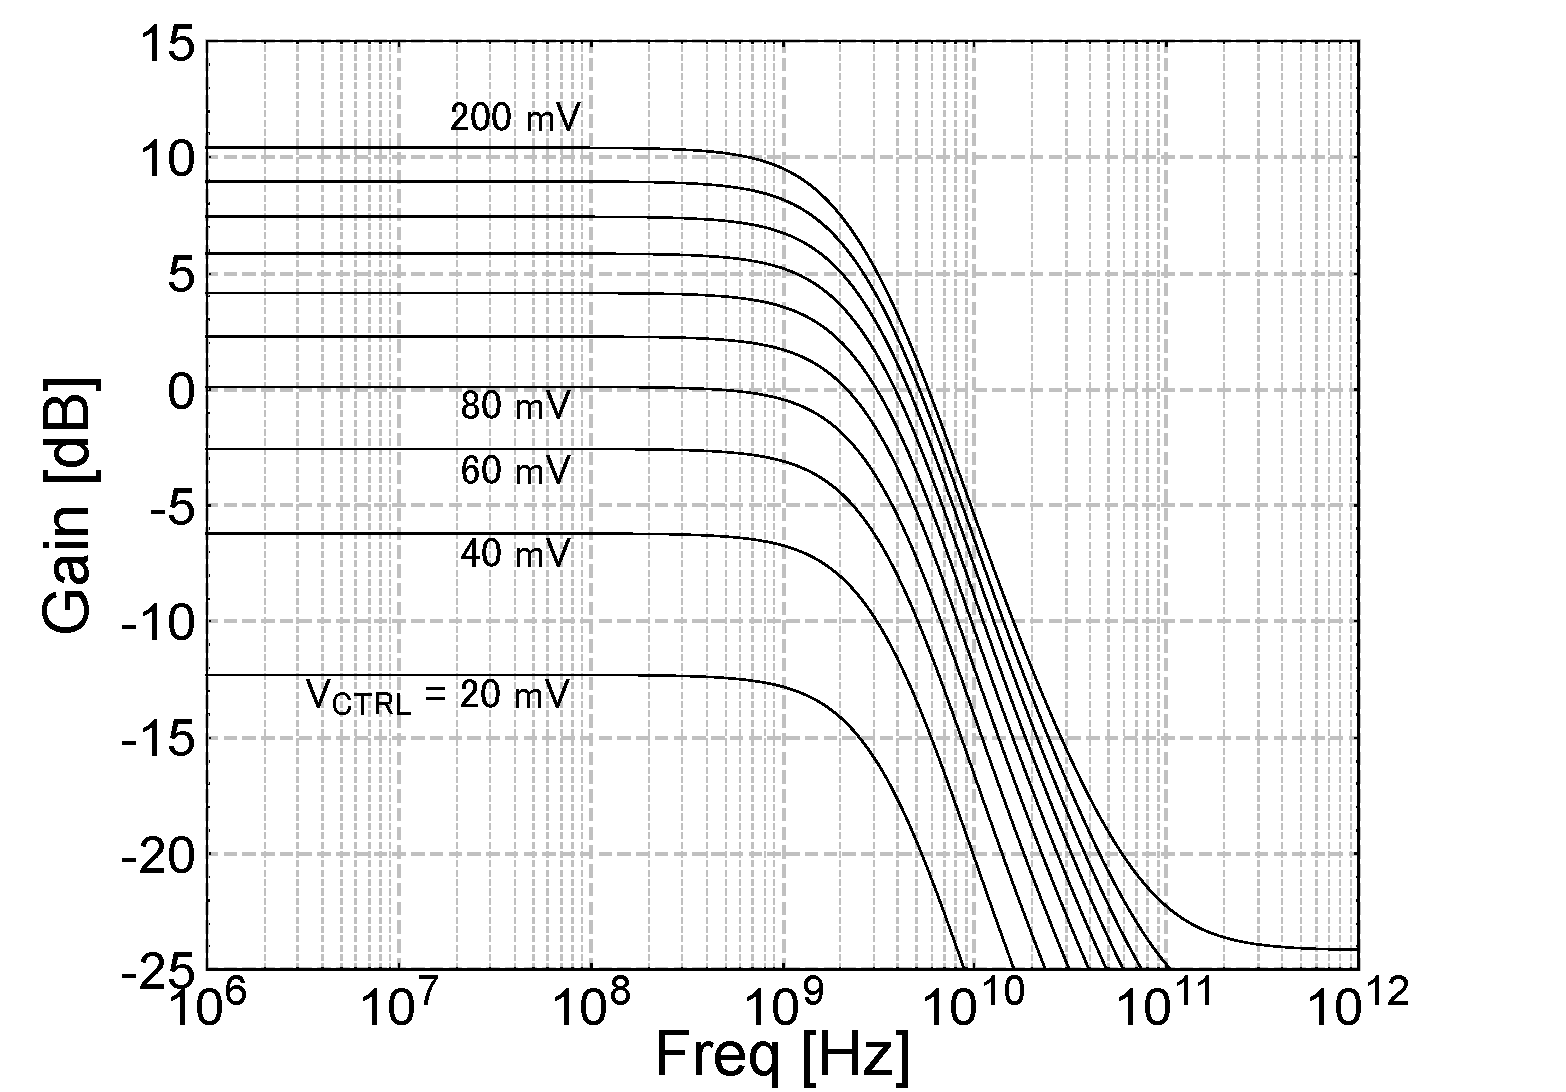
\includegraphics[width=0.99\textwidth]{figures/chapter3/previous_ac.pdf}
            \caption{ギルバート乗算回路の周波数特性}
            \label{fig:3_gilbert_ac}
        \end{figure}
        \begin{figure}[!b]
            \centering
            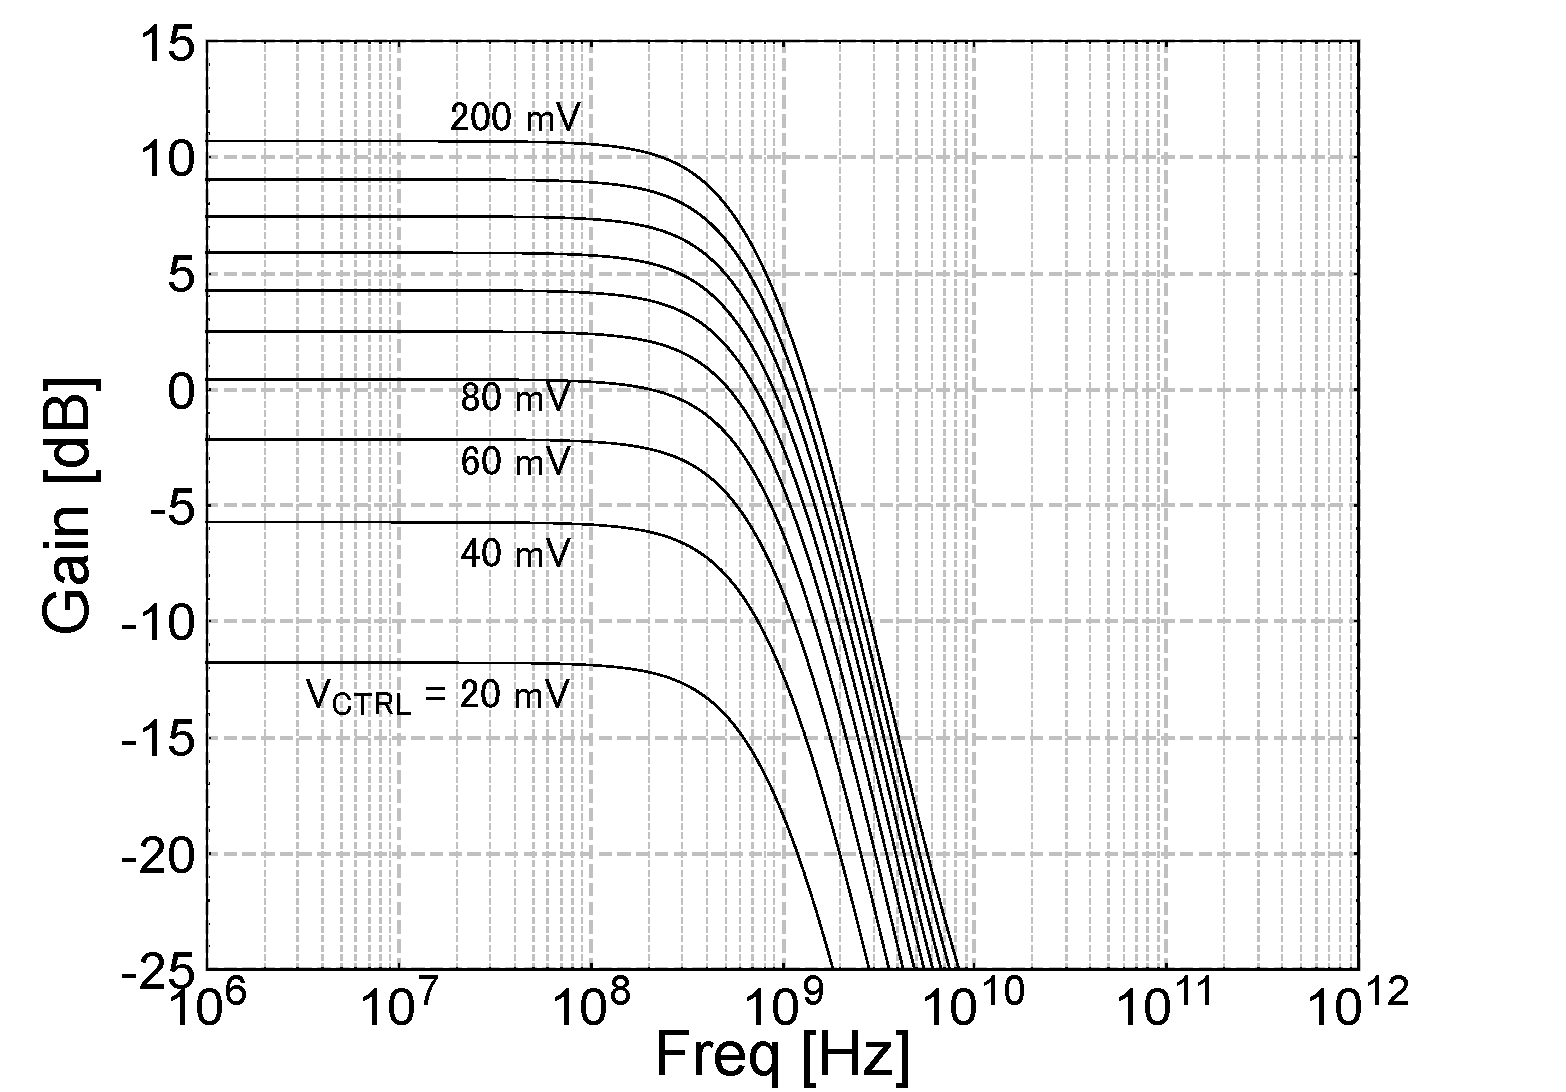
\includegraphics[width=0.99\textwidth]{figures/chapter3/folded_ac.pdf}
            \caption{折り返しカスコード型の周波数特性}
            \label{fig:3_folded_gilbert_ac}
        \end{figure}
        \clearpage
        今回の設計ではトランスコンダクタンスも揃っているので利得は同程度であるが、遮断周波数は1桁程度落ちてしまっている。本論文での目的はS/N比を向上させるために出力範囲を拡大することであるが、フォトニックリザバに用いることを想定すると周波数特性が構造的にギルバート乗算回路よりも悪化するのは避けたい。そこでpMOSFETを使用せずに信号の折り返しを行うことで出力範囲を拡大できるのではないかと考え、これを実現する回路を図\ref{fig:3_folded_mirror_gilbert}に示す。\par
        \begin{figure}[!b]
            \begin{center}
                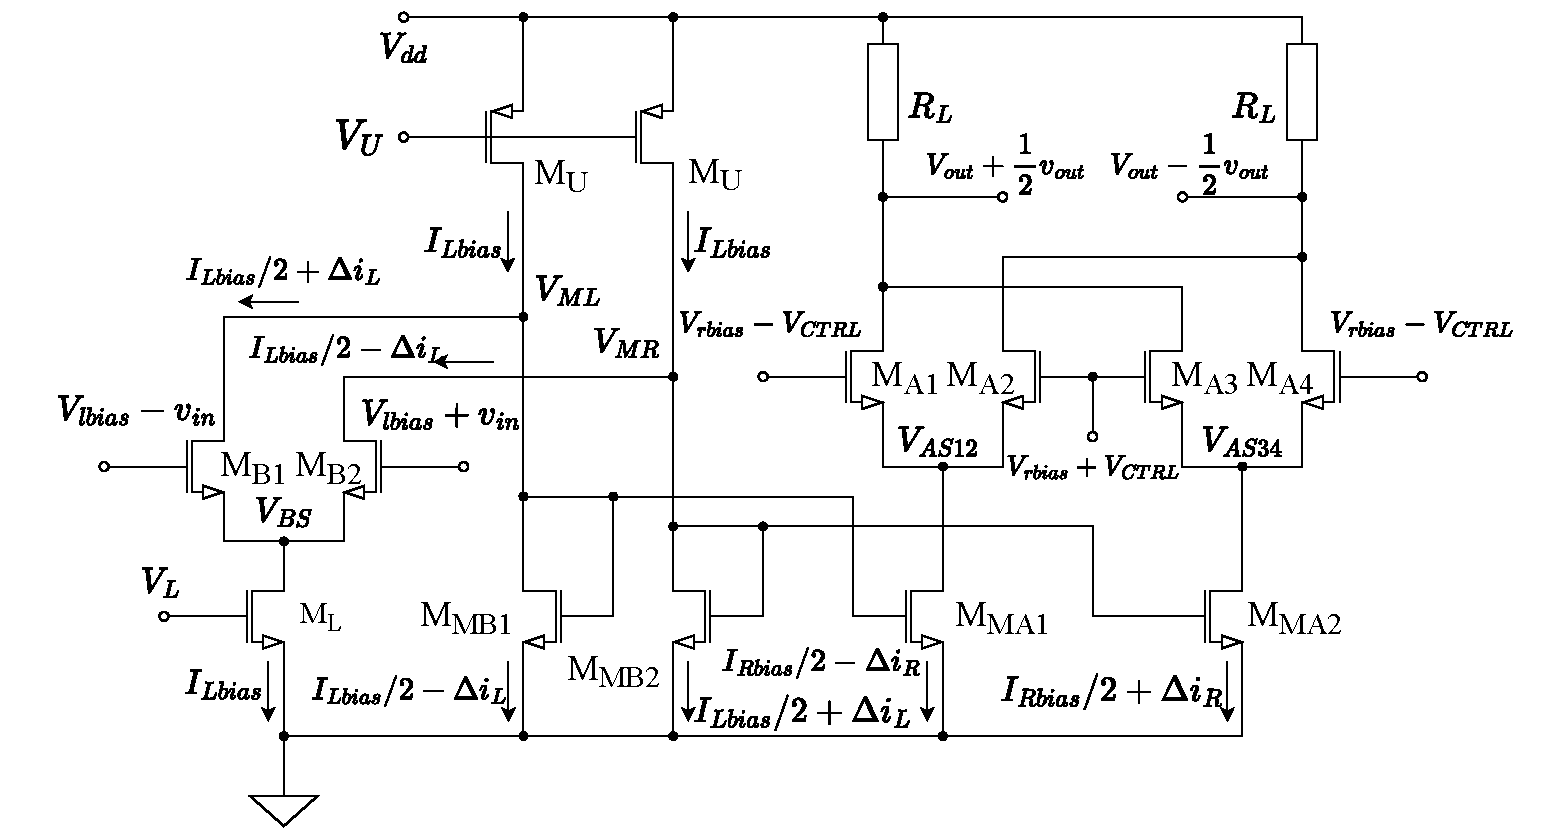
\includegraphics[width=0.99\textwidth]{figures/chapter3/NtoNFolded.pdf}
                \caption{カレントミラーを組み合わせた折り返し型乗算回路}
                \label{fig:3_folded_mirror_gilbert}
            \end{center}
        \end{figure}
        $\mathrm{M_{U},M_{L}}$はともに電流源として用いており、定電流$I_{Lbias}$を入力のMOSFETである$\mathrm{M_{B}}$とカレントミラーの参照電流を流す$M_{MB}$で分流する。これにより、入力の差動対によって$v_{in}$に比例した信号電流を符号を逆転させ$M_{MB}$に流す。カレントミラーのコピー側である$\mathrm{M_{MA}}$には$\mathrm{M_{MB}}$と$\mathrm{M_{MA}}$の形状比と$v_{in}$に比例した電流を流すことができる。これにより制御電圧を印加し、$\mathrm{M_{A}}$に流れるバイアス電流を変動させる。$\mathrm{M_{A}}$はゲート接地増幅回路であり、\ref{ch:gilbert_valiable_gm}節での議論からトランスコンダクタンスは$V_{CTRL}$に比例しており、負荷抵抗に流れる電流を$V_{in}$と$V_{CTRL}$に比例したものにすることができる。負荷抵抗によって電流を電圧に変換することができるという。このような想定の元、図\ref{fig:3_folded_mirror_gilbert}の構成を考えた。

    \section{小信号解析}
        前節では今回提案する構成によって乗算ができると考える理由を述べたが、本節では小信号解析により提案回路によって乗算が可能であることを示す。\par
        図\ref{fig:3_folded_mirror_gilbert}の小信号半回路を図\ref{fig:3_folded_mirror_half}に示す。
        \begin{figure}[!b]
            \centering
            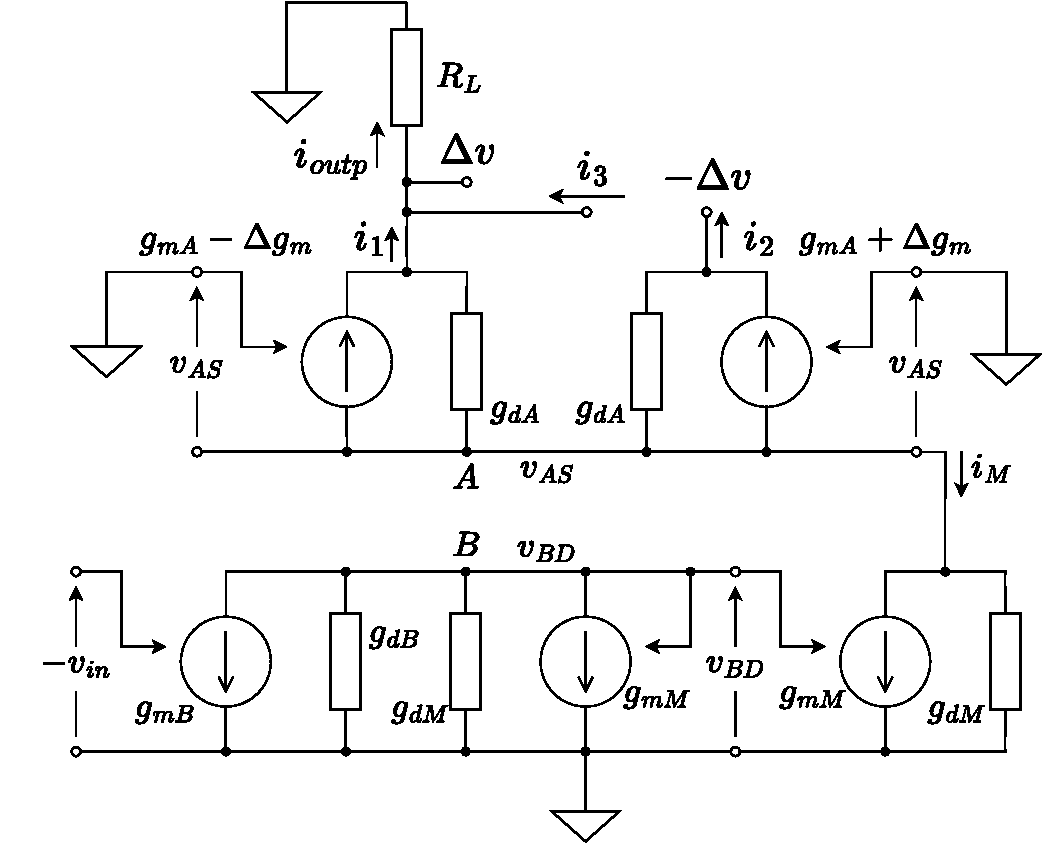
\includegraphics[width=125mm]{figures/chapter3/NtoNHalfDiffEqual.pdf}
            \caption{カレントミラーを組み合わせた折り返し型アナログ乗算回路の小信号半回路}
            \label{fig:3_folded_mirror_half}
        \end{figure}


    \section{出力範囲}


    \section{シミュレーションによる確認}




%    \begin{figure}[!b]
%        \centering
%        \includegraphics[width=0.9\textwidth]{figures/chapter}
%        \caption{}
%        \label{fig:3_}
%    \end{figure}

%    \begin{subequations}
%        \begin{empheq}[left={\empheqlbrace}]{align}
%        \end{empheq}        \label{eq:}
%    \end{subequations}
